\en{Let $ABC$ be an acute triangle with $BC > AC$. The perpendicular bisector of the segment $AB$ intersects the line $BC$ at $X$ and the line $AC$ at $Y$. Let $P$ be the projection of $X$ on $AC$ and let $Q$ be the projection of $Y$ on $BC$. Prove that the line $PQ$ intersects the segment $AB$ at its midpoint.

\textbf{Solution 1 (angle chasing, cylic quadrilaterals):} Introducing $M$ as the midpoint of $AB$, the exercise is equivalent to showing that $M$, $P$ and $Q$ are collinear. In order to do that, we will show that $\angle MPX+\angle XPQ=180^\circ$. We first note that there are a few cyclic quadrilaterals :
\begin{enumerate}
    \item $YQPX$ is cyclic, as $\angle XPY=90^\circ=\angle XQY$.
    \item $YQMB$ is cyclic, as $\angle BMY=90^\circ=\angle BQY$.
    \item $AMXP$ is cylic, as $\angle XMA=90^\circ=\angle XPA$.
\end{enumerate}
As $X$ is on the perpendicular bisector of $AB$, we have $XA=XB$ and $\angle MAX=\angle MBX\;(*)$.

Then,
\[
    \angle MPX\stackrel{\text{(c)}}{=} \angle MAX
    \stackrel{(*)}{=} \angle MBX
    = \angle MBQ
    \stackrel{\text{(b)}}{=} \angle MYQ
    = \angle XYQ
    \stackrel{\text{(a)}}{=} 180^\circ - \angle XPQ.
\]

\textbf{Solution 2 (more efficient than Solution 1):} There is a very similar way way to proceed, making use of only two of the aforementioned cyclic quadrilaterals, and that $YA=YB$ implies $\angle MYA=\angle MYB\;(*)$. This time, we show that $M$, $P$ and $Q$ are collinear by proving that $\angle XQP=\angle XQM$. Indeed,
\[
\angle XQP\stackrel{\text{(a)}}{=}\angle XYP=\angle MYA\stackrel{(*)}{=}\angle MYB\stackrel{\text{(b)}}{=}\angle MQB=\angle XQM.
\]

\textbf{Solution 3 (Menelaus and power of a point):} One could be tempted to show that $M$, $P$ and $Q$ are collinear by using Menelaus. We would need to prove that 
\[
\frac{AM}{MB}\cdot \frac{BQ}{QC}\cdot \frac{CP}{PA}\stackrel{?}{=}-1.
\]
Firstly, like in the other proofs, we note that $YQPX$ is cyclic as $\angle XPY=90^\circ=\angle XQY$. We will write $\omega$ for the circle $(YQPX)$. By Thales on a circle, its center is the midpoint of $XY$, in particular it lies on the perpendicular bisector of $AB$. As the power of a point with respect to $\omega$ is uniquely determined by its distance to this center, we have that $A$ and $B$ have the same power with respect to $\omega$, proving that 
\[
PA\cdot AY=XB\cdot BQ.
\]
The power of $C$ with respect to $\omega$ also yields that
\[
CX\cdot QC=CP\cdot YC.
\]
Combining these two equalities, we finally have that
\[
\frac{AM}{MB}\cdot \frac{BQ}{QC}\cdot \frac{CP}{PA}=-1\cdot \frac{BQ}{PA}\cdot \frac{CP}{QC}=-1\cdot \frac{AY}{XB}\cdot \frac{CX}{YC} =\frac{BM}{MA}\cdot \frac{AY}{YC}\cdot \frac{CX}{XB}=-1.
\]
In the last equality, we used Menelaus as $M$, $Y$ and $X$ are collinear.
\begin{center}
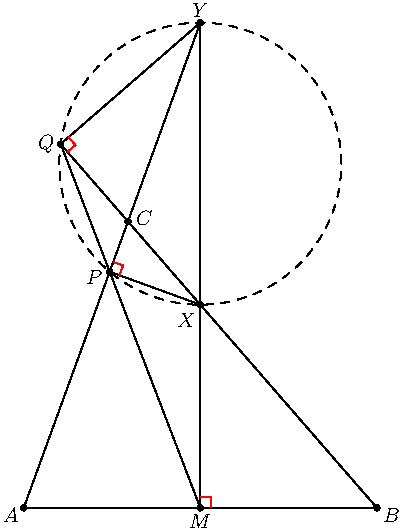
\includegraphics{g2fig}
\end{center}

\bigskip

\textbf{Marking Scheme - Solution 1 and 2}

\begin{itemize}
    \item 1P: Rewriting the statement in terms of angles, in a statement of the kind : 
    \begin{itemize}
        \item $\angle MPX+\angle XPQ=180^\circ$
        \item $\angle XQP=\angle XQM$
    \end{itemize}
    \item 3P: Showing that $YQPX$, $YQMB$ or $AMXP$ are cyclic (2P for one quadrilateral, 3P for two or three quadrilaterals)
    \item 1P: Proving that $\angle MAX=\angle MBX$, $\angle MAY=\angle MBY$ or that $\angle MYA=\angle MYB$.
    \item 2P: Conclude.
\end{itemize}

\textbf{Marking Scheme - Solution 3}

\begin{itemize}
    \item 1P: Stating the problem as a Menelaus equality.
    \item 1P: Proving that $YQPX$ is cyclic.
    \item 2P: Proving that $PA\cdot AY=XB\cdot BQ$.
    \item 1P: Proving that $CX\cdot QC=CP\cdot YC$.
    \item 2P: Conclude.
\end{itemize}
}

\de{Sei $ABC$ ein spitzwinkliges Dreieck mit $BC > AC$. Die Mittelsenkrechte der Seite $AB$ schneidet die Gerade $BC$ in $X$ und die Gerade $AC$ in $Y$. Sei $P$ die Projektion von $X$ auf $AC$ und sei $Q$ die Projektion von $Y$ auf $BC$. Beweise, dass die Gerade $PQ$ die Strecke $AB$ in ihrem Mittelpunkt schneidet.

\textbf{Lösung 1 (Winkeljagd, Sehnevierecke):}
Nach einführung von $M$ als der Mitpunkt von $AB$, genügt es zu zeigen, dass $P$, $Q$ und $M$ kolinear sind. Wir werden dies hier zeigen, indem wir beweisen, dass $\angle MPx + \angle XPQ = 180^\circ$ gilt.
Wir bemerken sazu zuerst ein paar Sehenenvierecke.
\begin{enumerate}
    \item $YQPX$ ist ein Sehnenviereck, da $\angle XPY = 90^\circ = \angle XQY$.
    \item $YQMB$ ist ein Sehnenviereck, da $\angle BMY = 90^\circ = \angle BQY$.
    \item $AMXP$ ist ein Sehnenviereck, da $\angle XMA = 90^\circ = \angle XPA$.
\end{enumerate}
Da nun $X$ auf der Mittelsenkrechten von $AB$ liegt, gilt $XA = XB$ und somit $\angle MAX = \angle MBX \;(*)$
Alles in allem gilt also:
\[
    \angle MPX\stackrel{\text{(c)}}{=} \angle MAX
    \stackrel{(*)}{=} \angle MBX
    = \angle MBQ
    \stackrel{\text{(b)}}{=} \angle MYQ
    = \angle XYQ
    \stackrel{\text{(a)}}{=} 180^\circ - \angle XPQ.
\]
Wie gewünscht.

\textbf{Lösung 2 (effizienter als Lösung 1):} Es gibt eine sehr ähnliche Vorgehensweis, die nur zwei der zuvorgenannten Sehnenvierecke benützt. Ebenfalls benutzen wir, dass $YA = YB$ bzw. $\angle MYA = MYB\;(*)$. Dieses Mal werden wir zeigen, dass $M$, $P$ und $Q$ kolinear sind, indem wir zeigen, dass $\angle XQP = XQM$. Wieder mit den obig genannten Sehnenvierecken gilt:

\[
\angle XQP\stackrel{\text{(a)}}{=}\angle XYP=\angle MYA\stackrel{(*)}{=}\angle MYB\stackrel{\text{(b)}}{=}\angle MQB=\angle XQM.
\]
Wie gewünscht.

\textbf{Lösung 3 (Menelaus und Potenz eines Punktes):} Man kann die kolinearität auch mit Menelaus zeigen. Dazu müsste man die folgende Gleichung verifizieren:
\[
\frac{AM}{MB}\cdot \frac{BQ}{QC}\cdot \frac{CP}{PA}\stackrel{?}{=}-1.
\]
Wie in den anderen beiden Lösungen, bemerken wir, dass $YQPX$ ein Sehnenviereck ist, da $\angle XPY = 90^\circ = \angle XQY$. Wir werden nun $\omega$ für den Kreis $(YQPX)$ schreiben. Nach dem Satz von Thales ist das Zentrum von $\omega$ der Mittelpunkt von $XY$, also vorallem auch auf der Mittelsenkrechten zu $AB$. Da die Potenz eines Punktes nur von der Distantz zum Kreismittelpunkt abhängt, ist die Potenz von $A$ und $B$ gleich bezüglich $\omega$, woraus folgt:
\[
PA\cdot AY=XB\cdot BQ.
\]
Betrachtet man auch noch die Potenz des Punktes $C$ erhält man
\[
CX\cdot QC=CP\cdot YC.
\]
Die beide Gleichungen zusammen ergeben nun
\[
\frac{AM}{MB}\cdot \frac{BQ}{QC}\cdot \frac{CP}{PA}=-1\cdot \frac{BQ}{PA}\cdot \frac{CP}{QC}=-1\cdot \frac{AY}{XB}\cdot \frac{CX}{YC} =\frac{BM}{MA}\cdot \frac{AY}{YC}\cdot \frac{CX}{XB}=-1.
\]
Wobei wir in der letzten Gleichung Menalaus auf $ABC$ und die Tatsache, dass $M$, $Y$ und $X$ kolinear sind, benutzt haben.

\begin{center}
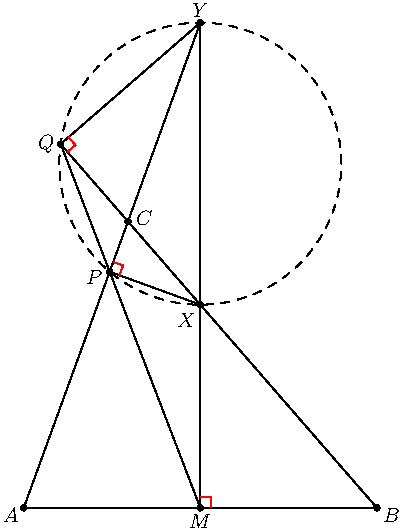
\includegraphics{g2fig}
\end{center}

\bigskip

\textbf{Marking Scheme - Lösung 1 und 2}
\begin{itemize}
    \item 1P: Umschreibung der zu beweisenden Aussage mit einer Winkelgleichung, wie beispielsweise:
    \begin{itemize}
        \item $\angle MPX+\angle XPQ=180^\circ$
        \item $\angle XQP=\angle XQM$
    \end{itemize}
    \item 3P: Zeigen, dass $YQPX$, $YQMB$ oder $AMXP$ Sehnenvierecke sind (2P für ein Sehenviereck, 3P für zwei oder drei Sehnenvierecke)
    \item 1P: Zeigen, dass $\angle MAX=\angle MBX$, $\angle MAY=\angle MBY$ oder dass $\angle MYA=\angle MYB$
    \item 2P: Den Beweis vollenden
\end{itemize}

\textbf{Marking Scheme - Lösung 3}

\begin{itemize}
    \item 1P: Das Problem zu einer Menelaus Gleichung umformen
    \item 1P: Zeigen, dass $YQPX$ zyklisch ist
    \item 2P: Zeigen, dass $PA\cdot AY=XB\cdot BQ$
    \item 1P: Zeigen, dass $CX\cdot QC=CP\cdot YC$
    \item 2P: Den Beweis vollenden
\end{itemize}
}




%french
\fr{Soit $ABC$ un triangle aigu avec $BC > AC$. La médiatrice du segment $AB$ coupe la droite $BC$ en $X$ et la droite $AC$ en $Y$. Soient $P$ la projection de $X$ sur $AC$ et $Q$ la projection de $Y$ sur $BC$. Montrer que la droite $PQ$ coupe le segment $AB$ en son milieu.

\textbf{Solution 1 (chasse aux angles, quadrilatères cycliques):} En posant $M$ comme le milieu d'$AB$, l'exercice est équivalent à montrer que $M$, $P$ et $Q$ sont colinéaires. Pour faire cela, nous allons montrer que $\angle MPX+\angle XPQ=180^\circ$. Nous notons d'abord qu'il y a quelques quadrilatères cycliques :
\begin{enumerate}
    \item $YQPX$ est cyclique, car $\angle XPY=90^\circ=\angle XQY$.
    \item $YQMB$ est cyclique, car $\angle BMY=90^\circ=\angle BQY$.
    \item $AMXP$ est cyclique, car $\angle XMA=90^\circ=\angle XPA$.
\end{enumerate}
Comme $X$ est sur la médiatrice d'$AB$, nous avons $XA=XB$ et $\angle MAX=\angle MBX\;(*)$.

Alors,
\[
    \angle MPX\stackrel{\text{(c)}}{=} \angle MAX
    \stackrel{(*)}{=} \angle MBX
    = \angle MBQ
    \stackrel{\text{(b)}}{=} \angle MYQ
    = \angle XYQ
    \stackrel{\text{(a)}}{=} 180^\circ - \angle XPQ.
\]

\textbf{Solution 2 (plus efficace que la Solution 1):} Il y a une façon très similaire de procéder, utilisant seulement deux des quadrilatères inscrits mentionnés plus haut, et le fait que $YA=YB$ implique $\angle MYA=\angle MYB\;(*)$. Cette fois, nous montrons que $M$, $P$ et $Q$ sont colinéaires en montrant que $\angle XQP=\angle XQM$. En effet, 
\[
\angle XQP\stackrel{\text{(a)}}{=}\angle XYP=\angle MYA\stackrel{(*)}{=}\angle MYB\stackrel{\text{(b)}}{=}\angle MQB=\angle XQM.
\]

\textbf{Solution 3 (Ménélaüs et puissance d'un point):} Nous pourrions être tentés de montrer que $M$, $P$ et $Q$ sont colinéaires avec Ménélaüs. Nous aurions besoin de
\[
\frac{AM}{MB}\cdot \frac{BQ}{QC}\cdot \frac{CP}{PA}\stackrel{?}{=}-1.
\]
Tout d'abord, comme dans les autres preuves, on note que $YQPX$ est cyclique comme $\angle XPY=90^\circ=\angle XQY$. Écrivons $\omega$ pour le cercle $(YQPX)$. Par le théorème de Thalés sur le cercle, son centre est le milieu de $XY$, en particulier il se trouve sur la médiatrice de $AB$. Comme la puissance d'un point par rapport à $\omega$ est uniquement déterminée par sa distance à ce centre, nous avons que $A$ et $B$ ont la même puissance par rapport à $\omega$, prouvant que
\[
PA\cdot AY=XB\cdot BQ.
\]
La puissance de $C$ par rapport à $\omega$ nous donne aussi que
\[
CX\cdot QC=CP\cdot YC.
\]
En combinant ces deux égalités, nous obtenons finalement que
\[
\frac{AM}{MB}\cdot \frac{BQ}{QC}\cdot \frac{CP}{PA}=-1\cdot \frac{BQ}{PA}\cdot \frac{CP}{QC}=-1\cdot \frac{AY}{XB}\cdot \frac{CX}{YC} =\frac{BM}{MA}\cdot \frac{AY}{YC}\cdot \frac{CX}{XB}=-1.
\]
Dans la dernière égalité, nous avont utilisé Ménélaüs comme $M$, $Y$ et $X$ sont colinéaires.
\begin{center}
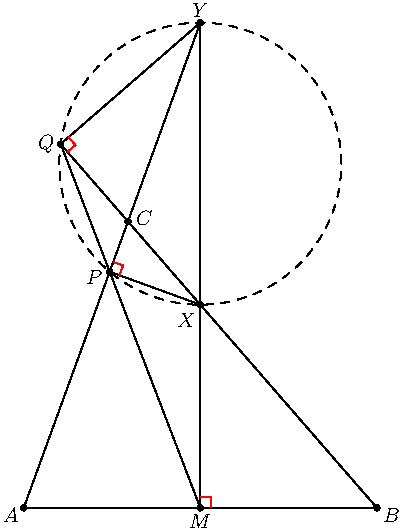
\includegraphics{g2fig}
\end{center}

\bigskip

\textbf{Marking Scheme - Solution 1 et 2}

\begin{itemize}
    \item 1P: Reformuler l'énoncé avec des angles, en une affirmation du type :
    \begin{itemize}
        \item $\angle MPX+\angle XPQ=180^\circ$
        \item $\angle XQP=\angle XQM$
    \end{itemize}
    \item 3P: Montrer que $YQPX$, $YQMB$ ou $AMXP$ sont cycliques (2P pour un quadrilatère, 3P pour deux ou trois quadrilatères)
    \item 1P: Montrer que $\angle MAX=\angle MBX$, $\angle MAY=\angle MBY$ ou que $\angle MYA=\angle MYB$.
    \item 2P: Conclure.
\end{itemize}

\textbf{Marking Scheme - Solution 3}

\begin{itemize}
    \item 1P: Reformuler l'énoncé comme une égalité de type Ménélaüs.
    \item 1P: Montrer que $YQPX$ est cyclique.
    \item 2P: Montrer $PA\cdot AY=XB\cdot BQ$.
    \item 1P: Montrer $CX\cdot QC=CP\cdot YC$.
    \item 2P: Conclure.
\end{itemize}
}
